% !TEX TS-program = XeLaTeX
% use the following command:
% all document files must be coded in UTF-8
\documentclass[portuguese]{textolivre}
% build HTML with: make4ht -e build.lua -c textolivre.cfg -x -u article "fn-in,svg,pic-align"


\journalname{Texto Livre}
\thevolume{18}
%\thenumber{1} % old template
\theyear{2025}
\receiveddate{\DTMdisplaydate{2025}{3}{13}{-1}} % YYYY MM DD
\accepteddate{\DTMdisplaydate{2025}{4}{16}{-1}}
\publisheddate{\DTMdisplaydate{2025}{6}{25}{-1}}
\corrauthor{Gustavo Ximenes Cunha}
\articledoi{10.1590/1983-3652.2025.58111}
%\articleid{NNNN} % if the article ID is not the last 5 numbers of its DOI, provide it using \articleid{} commmand 
% list of available sesscions in the journal: articles, dossier, reports, essays, reviews, interviews, editorial
\articlesessionname{articles}
\runningauthor{Oliveira et al.} 
%\editorname{Leonardo Araújo} % old template
\sectioneditorname{Daniervelin Pereira}
\layouteditorname{Saula Cecília}

\title{As novas fronteiras do dizível: a linguagem impolida contra figuras femininas das esferas política e judiciária}
\othertitle{The new boundaries of the sayable: impolite language against female figures in the political and judicial spheres}
% if there is a third language title, add here:
%\othertitle{Artikelvorlage zur Einreichung beim Texto Livre Journal}

\author[1]{Ana Larissa Adorno Marciotto Oliveira~\orcid{0000-0003-1857-0207}\thanks{Email: \href{mailto:adornomarciotto@gmail.com}{adornomarciotto@gmail.com}}}
\author[1]{Monique Vieira Miranda~\orcid{0000-0002-0935-5604}\thanks{Email: \href{mailto:nkmiranda@gmail.com}{nkmiranda@gmail.com}}}
\author[2]{Tímea Drinóczi~\orcid{0000-0002-7657-3572}\thanks{Email: \href{drinoczi.timea@gmail.com}{drinoczi.timea@gmail.com}}}
\author[1]{Gustavo Ximenes Cunha~\orcid{0000-0001-9953-1204}\thanks{Email: \href{gustavoxcunha@gmail.com}{gustavoxcunha@gmail.com}}}
\affil[1]{Universidade Federal de Minas Gerais, Faculdade de Letras, Belo Horizonte, MG, Brasil.}
\affil[2]{Universidade Federal de Minas Gerais, Faculdade de Direito, Belo Horizonte, MG, Brasil.}

\addbibresource{article.bib}
% use biber instead of bibtex
% $ biber article

% used to create dummy text for the template file
\definecolor{dark-gray}{gray}{0.35} % color used to display dummy texts
\usepackage{lipsum}
\SetLipsumParListSurrounders{\colorlet{oldcolor}{.}\color{dark-gray}}{\color{oldcolor}}

% used here only to provide the XeLaTeX and BibTeX logos
\usepackage{hologo}

% if you use multirows in a table, include the multirow package
\usepackage{multirow}

% provides sidewaysfigure environment
\usepackage{rotating}

% CUSTOM EPIGRAPH - BEGIN 
%%% https://tex.stackexchange.com/questions/193178/specific-epigraph-style
\usepackage{epigraph}
\renewcommand\textflush{flushright}
\makeatletter
\newlength\epitextskip
\pretocmd{\@epitext}{\em}{}{}
\apptocmd{\@epitext}{\em}{}{}
\patchcmd{\epigraph}{\@epitext{#1}\\}{\@epitext{#1}\\[\epitextskip]}{}{}
\makeatother
\setlength\epigraphrule{0pt}
\setlength\epitextskip{0.5ex}
\setlength\epigraphwidth{.7\textwidth}
% CUSTOM EPIGRAPH - END

% to use IPA symbols in unicode add
%\usepackage{fontspec}
%\newfontfamily\ipafont{CMU Serif}
%\newcommand{\ipa}[1]{{\ipafont #1}}
% and in the text you may use the \ipa{...} command passing the symbols in unicode

% LANGUAGE - BEGIN
% ARABIC
% for languages that use special fonts, you must provide the typeface that will be used
% \setotherlanguage{arabic}
% \newfontfamily\arabicfont[Script=Arabic]{Amiri}
% \newfontfamily\arabicfontsf[Script=Arabic]{Amiri}
% \newfontfamily\arabicfonttt[Script=Arabic]{Amiri}
%
% in the article, to add arabic text use: \textlang{arabic}{ ... }
%
% RUSSIAN
% for russian text we also need to define fonts with support for Cyrillic script
% \usepackage{fontspec}
% \setotherlanguage{russian}
% \newfontfamily\cyrillicfont{Times New Roman}
% \newfontfamily\cyrillicfontsf{Times New Roman}[Script=Cyrillic]
% \newfontfamily\cyrillicfonttt{Times New Roman}[Script=Cyrillic]
%
% in the text use \begin{russian} ... \end{russian}
% LANGUAGE - END

% EMOJIS - BEGIN
% to use emoticons in your manuscript
% https://stackoverflow.com/questions/190145/how-to-insert-emoticons-in-latex/57076064
% using font Symbola, which has full support
% the font may be downloaded at:
% https://dn-works.com/ufas/
% add to preamble:
\usepackage{fontspec}
\newfontfamily\Symbola{Symbola}
%\newfontfamily{\NotoEmoji}{NotoColorEmoji}[Renderer=Harfbuzz]
%\newfontfamily{\NotoEmoji} {NotoColorEmoji.ttf}[Renderer=Harfbuzz]
%\newfontfamily{\NotoEmoji}{Noto Color Emoji}
%\newfontfamily{\NotoEmoji}{/usr/share/fonts/truetype/noto/NotoColorEmoji.ttf} 

% in the text use:
% {\Symbola }
% EMOJIS - END

% LABEL REFERENCE TO DESCRIPTIVE LIST - BEGIN
% reference itens in a descriptive list using their labels instead of numbers
% insert the code below in the preambule:
%\makeatletter
%\let\orgdescriptionlabel\descriptionlabel
%\renewcommand*{\descriptionlabel}[1]{%
%  \let\orglabel\label
%  \let\label\@gobble
%  \phantomsection
%  \edef\@currentlabel{#1\unskip}%
%  \let\label\orglabel
%  \orgdescriptionlabel{#1}%
%}
%\makeatother
%
% in your document, use as illustraded here:
%\begin{description}
%  \item[first\label{itm1}] this is only an example;
%  % ...  add more items
%\end{description}
% LABEL REFERENCE TO DESCRIPTIVE LIST - END


% add line numbers for submission
%\usepackage{lineno}
%\linenumbers

\begin{document}
\maketitle

\begin{polyabstract}
\begin{abstract}
O fenômeno da linguagem de conflito tem sido investigado pelas lentes de diferentes estudiosos, por exemplo, na Sociologia e na Antropologia, nos Estudos Jurídicos, na Ciência Política, nos Estudos de Discurso e nas Mídias Sociais, entre outros. Neste artigo, adotamos uma perspectiva ancorada, principalmente, nas contribuições dos estudos da impolidez desenvolvidos no âmbito da pragmática linguística. Acreditamos que essa perspectiva permita compreender a correlação entre os ataques verbais contra grupos vulneráveis e a erosão discursiva da democracia. Para alcançar nosso objetivo, conduzimos um estudo multi-caso, envolvendo impolidez na esfera digital praticada contra figuras do mundo político e do judiciário. Especificamente, estudamos as características da impolidez usada em três episódios de ataque verbal envolvendo as deputadas Sâmia Bomfim e Erika Hilton e a ministra do STF, Cármen Lúcia Antunes Rocha. Os resultados alcançados no estudo sugerem que a ofensa verbal de gênero, no domínio cibernético, é alimentada, centralmente, pela fabricação, ou pela manutenção, do ciclo de ataques associado a um alvo comum, retratado como inferior. Os resultados revelam, assim, que o ciclo de agressão verificado nos três casos, ao obstruir o debate genuíno, afeta o tecido social como um todo, e não apenas as mulheres, ou as pessoas LGBT+.

\keywords{Impolidez \sep Ataques verbais \sep Redes sociais \sep Misoginia}
\end{abstract}

\begin{english}
\begin{abstract}
The phenomenon of conflictive language has been investigated through the lenses of different scholars, for example, in Sociology and Anthropology, Legal Studies, Political Science, Discourse Studies and Social Media, among others. In this paper, we adopt a perspective based mainly on the contributions of the models of impoliteness developed under the scope of linguistic pragmatics. We believe that this perspective allows us to understand the correlation between verbal attacks against vulnerable groups and the discursive erosion of democracy. To achieve our goal, we have conducted a multi-case study of impoliteness in the digital sphere enacted against figures from the political and judicial worlds. Specifically, we studied the characteristics of the impoliteness used in three episodes of verbal attacks involving two Congresswomen, Sâmia Bomfim and Erika Hilton, and a Supreme Court judge, Cármen Lúcia Antunes Rocha. The results suggest that gender-based verbal abuse in the cyber domain is largely fueled by the creation or maintenance of a cycle of attacks associated with a common target, portrayed as inferior. The results thus reveal that the cycle of aggression observed in the three cases, by obstructing genuine debate, affects the social fabric as a whole, and not just women or LGBT+ people.

\keywords{Impoliteness \sep Verbal attacks \sep Social media \sep Misogyny}
\end{abstract}
\end{english}
% if there is another abstract, insert it here using the same scheme
\end{polyabstract}

\section{Introdução}\label{sec-intro}
Nos últimos anos, ataques verbais, direcionados aos chamados grupos vulneráveis (ou minorizados) e a membros do judiciário, têm se apresentado com uma característica saliente do discurso político autoritário, visível em vários países, por exemplo, no Brasil, Alemanha, Áustria, Itália, Tailândia, Hungria e Estados Unidos. Embora o fenômeno possa ser identificado no discurso de líderes de outras afiliações políticas, ele é mais proeminente na extrema direita \cite{drinoczi-agnieska2022}. Para esses líderes e seus seguidores, as conquistas de alguns grupos representam uma ameaça aos direitos de uma maioria imaginária. É assim que mulheres, mesmo aquelas em posições influentes, são frequentemente constrangidas apenas por serem mulheres. Pessoas LGBT+\footnote{Usamos a sigla LGBT+ por entendermos que o símbolo de adição incorpore todos os grupos e identidades que a essa sigla se afiliam ou venham a se afiliar.} são alvo de ofensas por sua orientação sexual e descritas como transgressoras. Os ataques verbais direcionados a esses grupos são comumente produzidos por meio de insultos, provocações e falsas acusações.

O fenômeno da linguagem de conflito tem sido investigado pelas lentes de diferentes estudiosos, por exemplo, na Sociologia e na Antropologia, nos Estudos Jurídicos, na Ciência Política, nos Estudos de Discurso e nas Mídias Sociais, entre outros \cite{oliveira2024}. Neste artigo, adotamos uma perspectiva ancorada, principalmente, nas contribuições dos estudos da impolidez desenvolvidos no âmbito da pragmática linguística \cite{culpeper2010, culpeper2011}. Acreditamos que essa perspectiva permita compreender a correlação entre os ataques verbais contra grupos vulneráveis e a erosão discursiva da democracia. Mais especificamente, o intuito deste artigo é o de investigar como a impolidez pode ser usada, na esfera digital, como um meio para tentar desqualificar figuras públicas do mundo político e do judiciário.

Para alcançar nosso objetivo, o próximo item, “Linguagem impolida e indecorosa e o discurso populista contra grupos vulneráveis”, aborda os temas da desigualdade de gênero e misoginia no Brasil, bem como os ataques a pessoas LGBT+, enquanto uma questão ao mesmo tempo global e local. Em seguida, apresentamos os procedimentos metodológicos adotados neste estudo. Por fim, no item “Estudos multi-casos”, analisamos casos concretos de impolidez na esfera digital contra figuras do mundo político e do judiciário. Especificamente, o item trata das características da impolidez usada em três episódios de ataque verbal envolvendo as deputadas Sâmia Bomfim e Erika Hilton e a ministra do STF, Cármen Lúcia Antunes Rocha.

\section{Linguagem impolida e indecorosa e o discurso populista contra grupos vulneráveis}\label{sec-1}
No âmbito da pragmática linguística, os estudos da impolidez surgem da percepção de que as teorias clássicas da polidez (em especial, as propostas de \textcite{brown1987}, \textcite{leech1983} e \textcite{lakoff1975}, desenvolvidas na esteira dos estudos de \textcite{goffman1967}) não se ocupam do fato de que, em diversos contextos, os interlocutores não se valem de estratégias de polidez ou, em outros termos, deixam de amenizar o grau de agressividade de um ato de fala, utilizando-se de estratégias que protejam a face positiva (desejo de valorização) ou a negativa (desejo de autopreservação territorial) do próprio locutor ou do interlocutor. A partir sobretudo dos anos 1990, autores como \textcite{culpeper2011} e \textcite{bousfield2007} observam que, ao contrário, são vários os ambientes (escola, exército, mídia, etc.) em que os interlocutores são movidos pelo intuito de agravar os potenciais danos de atos de fala às faces envolvidas, valendo-se da linguagem para produzir insultos, xingamentos, ofensas, etc. É nesse movimento de reconhecer a impolidez como um fenômeno com inegáveis repercussões linguísticas que este estudo se insere\footnote{Maiores detalhes sobre a constituição do campo dos estudos da im/polidez podem ser consultados em \textcite{cunha2020}.}.

Um dos recursos empregados por líderes populistas, principalmente, mas não exclusivamente de extrema direita, para ostracizar opositores e atrair votos, é a linguagem impolida, que vem se tornando uma prática comum, tanto em ambiente físico quanto digital. Ao tomar a forma de insultos, insinuações e de falsas acusações, direcionadas comumente a minorias e ao sistema democrático como um todo, esse tipo de linguagem é formulada para vilipendiar, intimidar e silenciar indivíduos e grupos vistos como inimigos. O fenômeno é denominado “normalização da linguagem impolida e indecorosa”, e é considerado uma nova onda no debate político em vários países \cite{wodak2021culpeper}.

Nos Estados Unidos, por exemplo, durante sua presidência e além, Donald Trump questionou a legitimidade das instituições democráticas. Em um universo de 161 tweets, publicados no período de 1 de maio a 6 de maio de 2017, Trump promoveu ataques e críticas a instituições democráticas, à mídia comercial e a figuras públicas em pelo menos 58 deles \cite{koike2018}. No Brasil, conforme \textcite{oliveira2024} demonstraram, postagens de apoiadores de Bolsonaro circularam no período imediatamente anterior à eleição presidencial de 2022, questionando a legitimidade das urnas eletrônicas. Pauta bastante defendida pela extrema direita, o pleito pela retomada do voto de papel (voto impresso) provocou também a circulação de memes, contendo provocações aos ministros do STF, especialmente a Alexandre de Moraes, que presidiu o Tribunal Superior Eleitoral à época das eleições em 2022. Apesar de suas consideráveis contribuições para a erosão democrática e constitucional do país, Jair Bolsonaro não conseguiu se reeleger. Esse não foi o caso da Hungria, onde o líder de extrema direita, Viktor Orbán, conseguiu garantir a maioria necessária no parlamento, criar uma nova constituição iliberal e ser reeleito para quatro mandatos consecutivos como primeiro-ministro desde 2010 \cite{drinoczi-agnieska2022}.

Entre outras características, o discurso impolido e indecoroso tem o potencial de ``testar a estabilidade/flexibilidade das normas convencionais, oscilando entre o dizível e o indizível em contextos específicos'' \cite[p. 388]{wodak2021culpeper}. Esse discurso pode ser usado para contestar a legitimidade de eleições democráticas (como Trump fez), reproduzir rapidamente ideias autocráticas (como ocorreu na Índia de Modi) ou garantir a maioria constitucional mais de uma vez (como Viktor Orbán fez na Hungria). O exercício da impolidez também está associado, nesses casos, à ideia de divisão e de exclusão, bem como à criação de inimigos e ao consequente desrespeito aos direitos humanos, tais como a dignidade, a honra e a igualdade \cite{andrade2019, drinoczi-agnieska2022, drinoczi2022}.  

A propagação da impolidez no discurso populista de extrema direita também está associada ao fato de que esse tipo linguagem é atraente e profícuo em recursos linguísticos, tais como ``simplificação, polarização, intensificação, personalização, estereotipização e emocionalização'' \cite{wodak2021culpeper}, que são fáceis de reproduzir e disseminar \textit{online}. Ao desafiar os limites do dizível no ambiente político, a agressão verbal também é vista como um recurso para expressar raiva e frustração, particularmente em tempos de insegurança social. É também por meio da agressão verbal que líderes de extrema direita incitam seus seguidores a reafirmar uma alegada superioridade. Servindo como um epítome da desigualdade de poder e estratificação social, a crença na superioridade reside no cerne da retórica populista e é decisiva para ganhar seguidores nas mídias sociais, sancionando negativamente aqueles considerados transgressores, como mulheres e pessoas LGBT+, o que é feito em nome dos ``valores familiares tradicionais'', que são, em geral, brancos, coloniais e patriarcais.

Da mesma forma, é pelo exercício da impolidez linguística que líderes políticos populistas costumam manifestar opiniões extremas, de cunho sexista, racista, misógino e homotransfóbico. Esses ataques verbais muitas vezes alvejam líderes eleitos e figuras públicas influentes, transformando-os em transgressores. Particularmente em relação às mulheres, a ridicularização da aparência física \textit{(body shaming)} é uma maneira eficaz de ataque, empregado, quase sempre, para reduzir o valor de uma mulher a um patamar ficcional e inatingível de beleza \cite{oliveira2025}.

Na esfera digital, as estratégias de ridicularização da aparência física feminina são ainda mais proeminentes, devido aos recursos das plataformas de mídia social, como emojis, adesivos e links para vídeos remixados ou adulterados, que são frequentemente utilizados para imprimir um tom lúdico a postagens agressivas, contribuindo para sua disseminação viral. Ao empregar esses recursos, os usuários de mídias sociais também procuram mascarar a agressão verbal, fazendo-a soar como uma ``piada'' sem grandes consequências legais \cite{oliveira2025}. Essa conduta, quando praticada por líderes políticos e pessoas influentes, encoraja seus apoiadores a se comportarem da mesma maneira, dentro e fora do ambiente digital, em razão, principalmente, de oferecerem um apelo mais simples e emocional do que aquele em geral presente no discurso político tradicional. Como \textcite{zottola2022} chamam atenção, tais recursos demonstram que o apelo da fórmula discursiva da extrema direita reside ``precisamente em englobar qualquer coisa que possa ser vista como uma ameaça aos ideais nativistas'' \cite[p. 264]{zottola2022}. A agressão verbal desempenha, portanto, um papel fundamental na manutenção das práticas autoritárias de líderes iliberais e populistas e é vista como uma ferramenta decisiva para vilipendiar, intimidar e silenciar indivíduos ou grupos vulneráveis. Mais importante ainda, como apontamos anteriormente, esse tipo de discurso permanece prevalente mesmo quando líderes autoritários estão fora do poder.

A seguir, apresentamos os procedimentos metodológicos adotados neste estudo, antes de abordarmos separadamente os três episódios de ataque verbal envolvendo as deputadas Sâmia Bomfim e Erika Hilton e a ministra do Supremo Tribunal Federal (STF), Cármen Lúcia Antunes Rocha.


\section{Sobre os procedimentos metodológicos adotados na condução da pesquisa}\label{sec-2}

A análise multicasos, realizada neste trabalho e apresentada no próximo item\footnote{Os dados apresentados neste artigo provêm de um projeto maior intitulado ``Discurso Digitalmente Mediado da Extrema Direita no Brasil e seus Efeitos nos Direitos Humanos de Mulheres, Meninas e da Comunidade LGBT+'' (CNPq – Processo número 404672/2023-0) e compõem o CID -- Corpus de Impolidez Digital \cite{oliveira2024corpus}, disponível em \url{https://www.impolidezdigital.com}.}, é parte de um projeto maior. Como veremos, essa análise permitiu desvelar como/se os usuários de mídias digitais são moralmente compelidos a agirem em relação uns aos outros, tangenciando o conceito de reciprocidade linguística. Os ataques verbais, direcionados às deputadas Sâmia Bomfim e Erika Hilton, bem como à ministra Cármen Lúcia Antunes Rocha, foram retribuídos com ainda mais impolidez. Como o fenômeno da impolidez digital se sustenta por meio de múltiplos recursos, seu exame também requer que distintos instrumentos de análise sejam combinados, tanto de ordem qualitativa como quantitativa. Em razão desse desafio, nesta seção objetivamos descrever e comentar os procedimentos de nossa coleta e de análise de dados, na tentativa de informar pesquisadores interessados.

Após selecionarmos os episódios que repercutiram amplamente nas redes sociais, por meio da plataforma Google Trends, extraímos os comentários associados a postagens sobre o evento. No caso das duas deputadas, os comentários foram retirados de postagens em suas próprias redes sociais e de vídeos que apresentam o momento exato em que os ataques a ela ocorreram, cujos dados são analisados neste texto. No caso da ministra Cármen Lúcia Antunes Rocha, por não ter conta pública em rede social, os dados foram oriundos das postagens mais comentadas sobre o tópico e de excertos dos vídeos mais populares no YouTube.

Assim, após esse levantamento e seleção, os dados foram extraídos com auxílio das ferramentas para desenvolvedores (API) do Google e do Twitter. Todas as postagens foram formatadas em planilhas do Excel dentro das quais cada comentário estava associado a um \textit{link} de acesso ou captura de tela do conteúdo original, a fim de facilitar sua recuperação na hipótese de exclusão do conteúdo pelo usuário que o publicou. Especificamente quanto ao recorte de dados aqui apresentado, cabe ainda mencionar que o X/Twitter impõe um limite de 100 \textit{tweets}, que podem ser extraídos da sua plataforma de forma gratuita. Acima desse número, é necessário pagar um valor mensal. Diferentemente, o Google, até a data da publicação deste material, não monetiza em cima dos dados abertos ao público, quando utilizados para fins acadêmicos. A Tabela \ref{tab-1} apresenta os números de comentários extraídos de cada plataforma, totalizando 10.441 postagens. Desse total, 31,3\% das postagens continham ocorrências de impolidez, seja ela dirigida explicitamente às deputadas e à ministra, ou a outras figuras políticas e entidades a elas associadas de alguma forma.

%----CÓDIGO DA TABELA 1 ----%
\begin{table}[h!]
\centering
\begin{threeparttable}
\caption{Total de comentários analisados em cada plataforma.}\label{tab-1}
\begin{tabular}{lrrrrrr}
\toprule
 & \multicolumn{3}{c}{YouTube} & \multicolumn{3}{c}{X/Twitter} \\
\cmidrule(lr){2-4} \cmidrule(lr){5-7}
 & Total & Impolidos & \% & Total & Impolidos & \% \\
\midrule
Dep. Sâmia Bomfim & 494 & 339 & 68{,}62 & 600 & 81 & 13{,}50 \\
Dep. Érika Hilton & 6.665 & 1.993 & 29{,}90 & 100 & 4 & 4{,}00 \\
Min. Cármen Lúcia Antunes Rocha & 2.282 & 829 & 36{,}33 & 300 & 29 & 9{,}67 \\
\midrule
Total & 9.441 & 3.161 &  & 1.000 & 114 &  \\
\bottomrule
\end{tabular}
\source{Corpus de Impolidez Digital - CID \cite{oliveira2024corpus}.}
\notes{Os comentários impolidos do X/Twitter e do YouTube referem-se unicamente àqueles dirigidos às deputadas e à ministra.}
\end{threeparttable}
\end{table}


Ao iniciarmos a análise manual de identificação e de classificação das ocorrências de impolidez, o material ofensivo às deputadas e à ministra foi minuciosamente categorizado. Com esses dados, foi possível gerar listas de palavras e de \textit{n-grams} (conjuntos de palavras) mais frequentes, utilizando a plataforma Sketch Engine\footnote{SKETCH ENGINE. Disponível em: \url{https://www.sketchengine.co.uk/}. Acesso em: 22 nov. 2024.}, a fim de melhor compreender os dados quantitativamente, em conjunto com a análise pormenorizada feita em cada etapa. Ao analisarmos o material, foi possível observar, com precisão, os termos mais frequentes que representavam fórmulas de impolidez, tais como os insultos, e também a quem esses termos eram dirigidos\footnote{Embora os parâmetros avaliativos de emotividade, que refletem a desaprovação dos usuários em relação às figuras públicas, sejam uma característica comum dos comentários analisados -- e, portanto, dialoguem com a Teoria da Avaliatividade \cite{martin2005} --, nosso foco aqui recai sobretudo no fato de que eles podem conter itens lexicais específicos, intrinsecamente avaliativos, ou surgir de forma implícita a partir de trechos que não contenham lexemas explicitamente avaliativos. Em ambos os casos, há uma implicação de impolidez em geral também compreendida como tal pelo falante comum da língua portuguesa. (Agradecemos a um dos avaliadores anônimos apontar o interesse da aproximação do nosso estudo e do sistema de \textcite{martin2005}, aproximação que poderá ser objeto de desenvolvimento em estudos futuros).}.

Após essa etapa, consideramos que, em pesquisas envolvendo grandes conjuntos de dados, mesmo que alguns filtros e mecanismos de busca sejam usados para extrair o conteúdo preliminar, o núcleo central do estudo é, muitas vezes, examinado manualmente, ainda que em forma de amostragem aleatória, conforme o caso. Assim, na referida etapa de análise manual, incorporamos uma abordagem mista de exame de dados \cite{unger2016}, incluindo componentes visuais (como \textit{memes} e \textit{emojis}) e verbais. Com essa escolha de metodologia, conforme já mostrado nos exemplos discutidos anteriormente, buscamos determinar se/como os recursos das plataformas digitais facilitam a disseminação de visões misóginas e transfóbicas, feitas por líderes de extrema direita e/ou por seus potenciais apoiadores ao exercerem impolidez linguística.

Com relação às questões éticas, baseando-se em estudos de \textcite{dynel2023} sobre pesquisa em impolidez em diferentes mídias sociais e seguindo as regras da \textit{Association of Internet Researchers}, as plataformas de redes sociais são consideradas ambientes públicos, nos quais os usuários conhecem o amplo alcance de suas publicações. Desse modo, os dados coletados podem ser usados para diferentes fins, incluindo estudos acadêmicos, especialmente por terem sido extraídos de modo não-intrusivo, por exemplo, sem a necessidade de pagar taxas quebrando a barreira da privacidade definida pelo usuário. Apesar disso, todas as marcas de autoria foram removidas das postagens, uma vez que o foco do trabalho está no conteúdo e não no autor dos comentários, com exceção das postagens feitas pelas figuras políticas envolvidas nos casos em questão.

\section{Estudos multi-casos}\label{sec-3}
Este item centra-se em três episódios de ataque verbal envolvendo as deputadas Sâmia Bomfim e Erika Hilton, bem como a ministra do STF, Cármen Lúcia. Os ataques verbais aqui analisados foram perpetrados contra elas por líderes políticos de extrema direita e proferidos durante discursos públicos que viralizaram nas redes sociais. Devido a restrições de espaço, selecionamos 10 postagens de duas plataformas digitais (a saber, X/Twitter e YouTube), associadas a cada uma dessas três figuras públicas. As postagens são mostradas na ordem de sua aparição nos \textit{threads} (fios) ou retiradas aleatoriamente dos dados e visam a proporcionar um ponto de vista privilegiado sobre os ataques baseados em gênero, associados ao esforço coletivo de menosprezar mulheres e pessoas LGBT+, mesmo quando ocupam cargos eletivos ou posições influentes.

\subsection{Deputada Sâmia Bomfim}\label{sec-3.1}
A deputada Sâmia Bomfim (Partido Socialismo e Liberdade -- PSOL) foi agraciada em 2023 com o primeiro lugar no Prêmio Congresso em Foco, que prestigia os melhores deputados e senadores por júri popular e de especialistas. Na premiação, o segundo lugar foi destinado à Erika Hilton (PSOL). O reconhecimento do trabalho das deputadas, juntamente com os dados quantitativos elencados (e detalhados na sequência) por nós nesta obra, justificam a seleção das duas deputadas para a discussão que pretendemos fazer aqui.

Como um de nossos objetivos é investigar características do metadiscurso de impolidez, primeiramente foi necessário determinar se houve e quais foram os ataques verbais às deputadas, de modo a selecionar aqueles com maior repercussão. Assim, utilizando a ferramenta Google Trends\footnote{GOOGLE TRENDS. Disponível em: \url{https://trends.google.com.br/trends/}. Acesso em: 24 nov. 2024.}, foi possível monitorar as buscas dos usuários pelos nomes das deputadas (e também da ministra), a fim de observar quando houve maior interesse do público em relação a elas. A partir desse passo, procuramos identificar o evento gerador do aumento de interesse dos usuários pelas deputadas com a finalidade de entrecruzar esse interesse com a repercussão gerada pelos possíveis ataques verbais a elas. Os picos de interesse, indicados na Figura \ref{graf-1}, ilustram o interesse do público em Sâmia Bomfim.

\begin{figure}[h!]
\centering
\begin{minipage}{.95\textwidth}
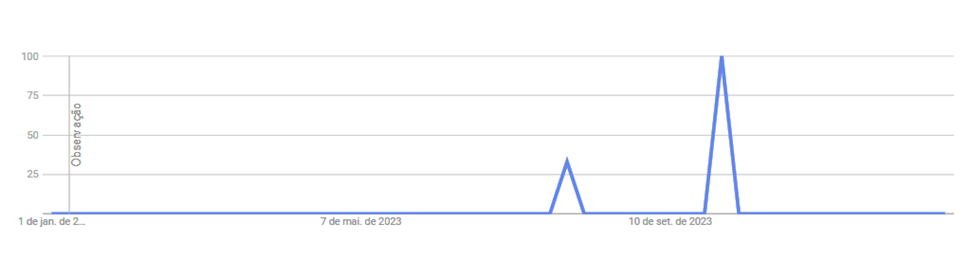
\includegraphics[width =\textwidth ]{Fig1.png}
\caption{Pico de interesse em Sâmia Bomfim.}
\label{graf-1}
\source{Plataforma \textit{online} Google Trends.}
\end{minipage}
\end{figure}

Como pode ser verificado na Figura \ref{fig-1}, o maior ponto de interesse público em Sâmia Bomfim ocorreu entre 1 e 5 de outubro de 2023, período que coincidiu com a circulação de notícias sobre um episódio trágico da vida pessoal da deputada (o assassinato de seu irmão em 5 de outubro de 2023). Como este evento específico não estava relacionado à presente pesquisa, escolheu-se para a análise o segundo pico, que ocorreu entre 30 de julho e 5 de agosto, quando o deputado Tenente-Coronel Luciano Zucco (Partido Liberal – PL), em pronunciamento no parlamento durante uma sessão na CPI do MST, se dirigiu à Sâmia pedindo para que ela se ``acalmasse'' e acrescentou: ``Está nervosa, deputada? Quer um remédio ou um hambúrguer?''.

A reprodução das observações de Zucco viralizou nas redes sociais, particularmente no YouTube, onde os dois vídeos mais repercutidos alcançaram mais de 25 mil visualizações e 500 comentários no momento da coleta de dados. Da mesma forma, no Twitter, o evento gerou cerca de 13.000 comentários/\textit{tweets} sobre o assunto, 12.000 repostagens de \textit{tweets} e 73 mil curtidas tanto em \textit{posts} da deputada quanto dos deputados Zucco e Ricardo Salles (PL), que estava presente na sessão, ao lado do colega de partido, e comentou o assunto em suas redes.

Após selecionar os episódios com ampla repercussão em mídias sociais, extraímos os comentários dos usuários nas publicações mencionadas no X/Twitter e no YouTube usando a ferramenta para desenvolvedores (API) do X/Twitter e do Google. As postagens foram, então, analisadas quanto à presença de marcas de impolidez verbal, como asserções negativas, perguntas desafiadoras, sarcasmo, críticas, insultos e insinuações \cite{culpeper2011}. Todo material linguístico, assim como o \textit{link} e a cópia da mensagem original, em caso de ser apagada, foram salvos em planilhas de Excel.

Conforme a Figura \ref{graf-2} atesta, nos dados coletados sobre a deputada Sâmia Bomfim, a forma mais usada para exercer impolidez jocosa foi o uso do sinal ``kkk'' e o emoji de riso ``{\Symbola 😂}''.
Esse dado é corroborado pela lista de itens (palavras e não-palavras, como sinais de pontuação e \textit{hashtags}) mais frequentes no CID, gerada com auxílio do programa online Sketch Engine. Nessa lista, o item mais frequente foi o emoji ``chorando de rir'' ({\Symbola 😂}).
A frequência desse item superou em três vezes o número de ocorrências da primeira palavra gramatical mais frequente em todo o corpus (``que'') e em seis vezes a primeira palavra lexical mais empregada (``hambúrguer'').

\begin{figure}[h!]
\centering
\begin{minipage}{.70\textwidth}
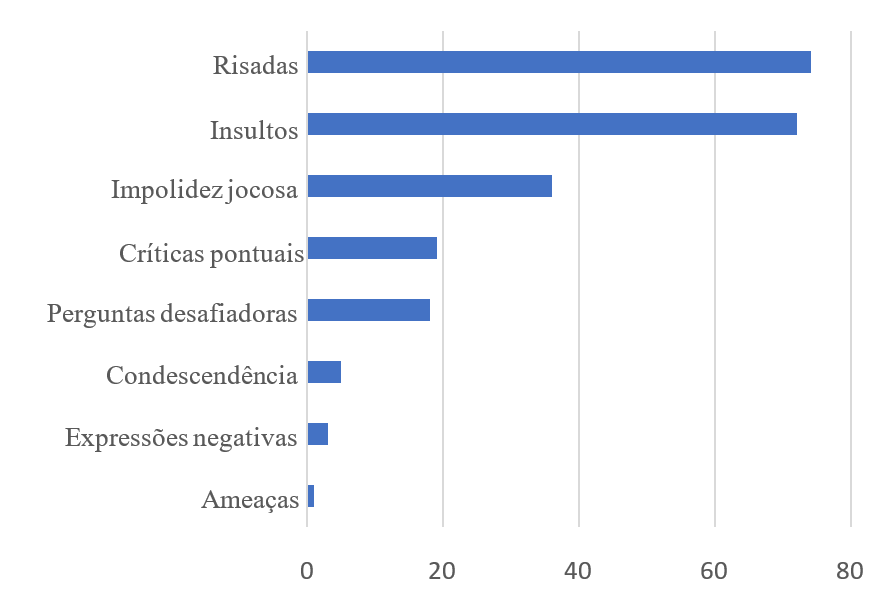
\includegraphics[width=\textwidth]{Fig2.png}
\caption{Tipos de ataques mais frequentes perpetrados contra a deputada Sâmia Bomfim.}
\label{graf-2}
\source{Elaboração própria.}
\end{minipage}
\end{figure}

\begin{figure}[h!]
\centering
\begin{minipage}{.5\textwidth}
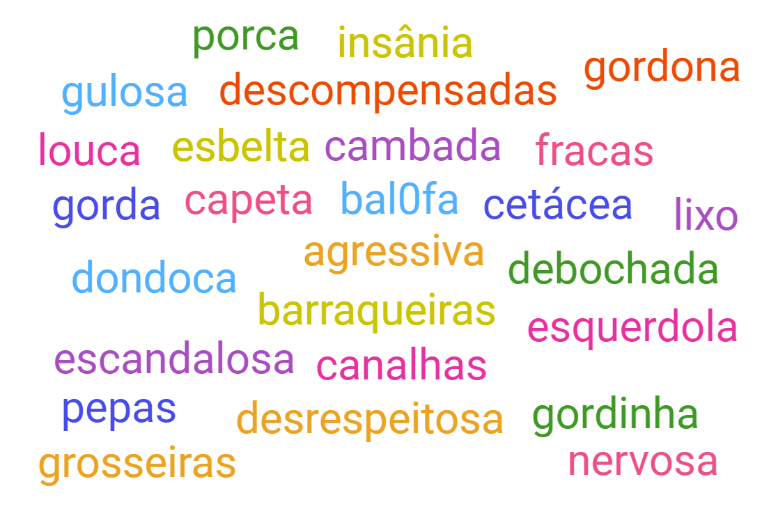
\includegraphics[width=\textwidth]{Fig3.png}
\caption{Termos ofensivos dirigidos à deputada Sâmia Bomfim.} \source{Autores, com auxílio dos programas Sketch Engine para fornecer as listas de palavras mais frequentes e Venngage\footnotemark para representar a lista em forma de nuvem de palavras.}
\label{fig-1}
\end{minipage}
\end{figure}
\footnotetext{VENNGAGE. Disponível em: \url{https://pt.venngage.com/}. Acesso em 11 set. 2024.}


Especificamente quanto aos insultos empregados, embora a maioria deles esteja associada à prática de \textit{body shaming} contra a deputada, o conjunto de dados foi marcado pela criatividade linguística, o que pode ser observado na Figura \ref{fig-1}, que traz alguns dos termos ofensivos dirigidos à deputada, como ``hamburgão'', ``gordona'', ``leitoa'' e ``balofa'', que representam expressões de impolidez na língua portuguesa brasileira, reconhecidas como tal pela maioria dos falantes, e comumente empregadas para insultar as pessoas por sua alegada aparência física fora do padrão.

Os insultos à deputada Sâmia Bomfim não se limitaram, no entanto, ao tema da aparência física. Eles também alvejaram a sua personalidade, caráter e equilíbrio mental, como pode ser observado pelo emprego de termos tais como ``porcaria'', ``louca'', ``barraqueira'' e ``mimizenta''. Além disso, registrou-se a frequente acusação de que a deputada ``tumultua'' as sessões e de que se ``vitimiza''. Em particular, acerca do termo ``vitimiza'', empregado nas postagens ofensivas contra a deputada Sâmia Bomfim, a ``vitimização terciária'' é um termo reconhecido no meio jurídico e empregado no âmbito da misoginia e da violência contra mulheres para caracterizar situações em que a vítima de violência não é acolhida (seja por familiares, amigos ou pela sociedade em geral), e é encorajada a não denunciar o crime (ou abuso) às autoridades. Também fazem parte desse processo as tentativas de descredibilizar e ridicularizar a mulher, por meio, como é o caso em nossos dados, de postagens ofensivas nas redes sociais, publicadas com o intuito de desqualificá-la e de enfraquecer suas demandas.

Como já observamos, líderes autoritários e seus seguidores costumam direcionar insultos a mulheres para agradar seus apoiadores e ganhar votos. Assim, ao remover os limites de conduta verbal polida, licenciar ou até defender a impolidez, o despudor verbal se torna uma prática importante. Sob essa perspectiva, o uso de \textit{body shaming} e da desqualificação moral servem como recursos úteis para líderes populistas atacarem seus rivais e reafirmarem a retórica ``nós'' versus ``eles''. Nessa lógica, a figura feminina é, muitas vezes, caracterizada como inferior, podendo ser criticada por sua aparência física, caráter e competência. Esses elementos podem ser observados na amostra seguinte de dez comentários aleatórios, retirados de nossos dados do X/Twitter:

\medskip
\begin{enumerate}
\item MC Donald's ou Burger King?
\item Mas quer hambúrguer ou pizza?
\item Vc deu uma emagrecida! Parece que tá só com 150kg agora!
\item Esses Hambúrgueres não passarão
\item Pelo tamanho... esse passarinho não voa... ROLA MORRO ABAIXO {\Symbola 🤣🤣🤣🤣🤣🤣}
\item Seja mulher e assuma o que vc faz com outras pessoas, fica feio essa vitimização pois está tudo gravado, aliás se alguém oferecer um hambúrguer eu fico muito feliz {\Symbola 🤣}
\item Sua fome insaciável por hambúrgueres está te deixando cada vez mais doida... Como mais antes de ir às comissões da Câmara dos Deputados. Fica a dica. Outra coisa... Emagreça, você parece uma Kombi. Abraço.
\item Parabéns Zucco, só disse verdades
\item Pq vc não fala que ela não respeita ninguém e agride todos que pensam diferente?
\item E sim, ela é nervosa e gorda. O que há de falso nisso?
\end{enumerate}
\medskip

Como os exemplos (1-10) mostram, as insinuações e as provocações direcionadas a Sâmia Bomfim foram comumente ancoradas em modelos imaginários de ``beleza'' e ``sensualidade''. Tais modelos parecem ressoar em certos setores da sociedade, como indicam os exemplos (3), (5), (7) e (10), que reproduzem esses padrões e os legitimam. Nessas mensagens, a prática do \textit{body shaming} e do \textit{fat shaming} foi evocada de forma explícita, fazendo referências à aparência física da deputada, por meio de insultos e do uso de expressões consideradas depreciativas em língua portuguesa (``feia'', ``gorda'') \cite{oliveira2022}.

Além disso, a capacidade mental da deputada Sâmia Bomfim foi frequentemente depreciada, como mostram os exemplos (7) e (10). Nesses exemplos, a deputada é negativamente descrita como ``louca'' e ``nervosa'', respectivamente, implicando que ela seja irracional, excessivamente emocional e facilmente agitável, avaliações negativas comumente atribuídas a mulheres, e que ecoam as observações feitas pelo deputado Zucco (``Está nervosa, deputada? Quer um remédio ou um hambúrguer?''). Todos esses estereótipos femininos, empregados para atacar Sâmia Bomfim, ajudam a forjar uma imagem negativa das mulheres em geral e sugerem a estratégia de transformar a vítima em algoz \cite{wodak2018}, como pode ser atestado mais claramente no exemplo (6), em que a deputada é explicitamente acusada de vitimização.

Nesses exemplos, também é possível depreender que a impolidez jocosa, associada ao sarcasmo, deboche e comentários com efeito humorísticos, foi utilizada nos ataques contra a deputada com a finalidade de antecipar a evasão de culpa em caso de um processo legal por assédio moral, difamação ou violência de gênero. Nesses casos, a alegação de que as mensagens eram meramente ``lúdicas'' pode, eventualmente, servir como tentativa de transformar a agressão verbal em simples ``brincadeirinha'', sem maiores consequências. Esse recurso pode ser atestado nos exemplos (5) e (6), em que o emoji ``{\Symbola 😂}
– chorando de rir'' é usado para conferir um tom sarcástico às postagens. Nesses exemplos, o sarcasmo e a zombaria sugerem, ainda, uma tentativa de legitimar a agressão verbal e desferir críticas amargas, como aquelas identificadas no exemplo (7), entre outros.

Nos dados sobre a deputada Sâmia Bomfim, entre os recursos utilizados para manifestar impolidez, as perguntas desafiadoras \cite{culpeper2010, culpeper2011} também se mostraram fundamentais, como demonstram os exemplos (1), (2), (9) e (10). Esse tipo de pergunta geralmente espelha desprezo, assimetria de conhecimento e desequilíbrio de poder. Elas emanam do papel epistêmico comumente atribuído aos falantes quando avaliam comportamentos sociais por meio de uma conduta verbal inquisitiva \cite{raymond2006, tantucci2023}. Como não se trata de perguntas genuínas, elas são empregadas quando o locutor tenta impor suas crenças, opiniões e avaliações aos ouvintes/leitores (``Mas quer hambúrguer ou pizza?'', exemplo 2). Em nossos dados, as perguntas desagradáveis funcionaram como recursos de provocação, atribuindo uma orientação política à discussão, já que evocavam o discurso do deputado Tenente-Coronel Zucco contra a deputada Sâmia Bomfim.


\subsection{Deputada Erika Hilton}\label{sec-3.2}

Quanto à deputada Erika Hilton, o procedimento de levantamento de eventos e notícias mais populares realizado anteriormente foi reproduzido para coletar dados sobre a deputada nas redes digitais. Em 2023, como pode ser observado na Figura \ref{graf-3}, o pico de interesse público em Erika ocorreu entre 27 de agosto e 2 de setembro de 2023. No vídeo associado a este episódio, datado de 30 de agosto de 2023, Hilton rebateu a deputada Coronel Fernanda (PL) após esta ter afirmado, em um discurso público no Parlamento Brasileiro, que mulheres trans privavam ``mulheres reais'' de seus direitos. No X/Twitter, o vídeo alcançou aproximadamente 4,2 milhões de visualizações e mais de 2,8 mil respostas. As declarações públicas de Erika Hilton se tornaram um dos tópicos mais comentados na plataforma, ocupando essa posição por cerca de 8 horas. O vídeo também viralizou em outras mídias digitais. No YouTube, os dois vídeos mais populares sobre o tema obtiveram aproximadamente 731 mil visualizações no total, atraindo mais de 6 mil comentários, que foram coletados para a presente análise. A Figura \ref{graf-3} mostra o interesse público em Erika Hilton, após a circulação dos vídeos nas plataformas digitais.

\begin{figure}[h!]
\centering
\begin{minipage}{.90\textwidth}
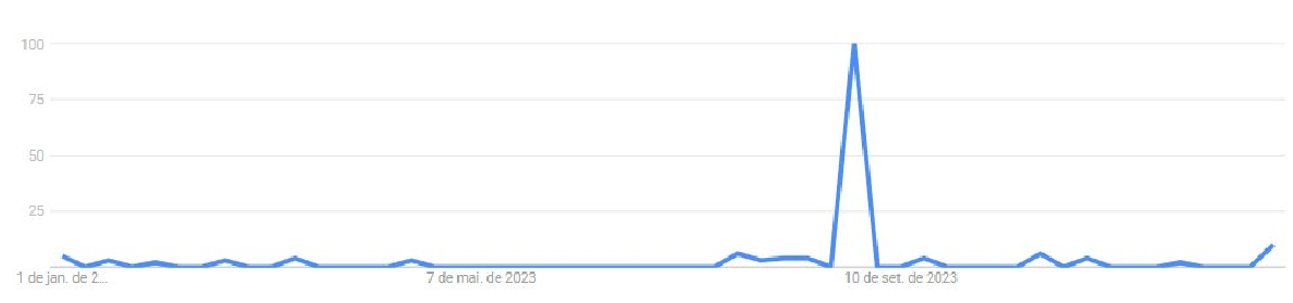
\includegraphics[width =\textwidth]{Fig4.png}
\caption{Pico de interesse público em Erika Hilton.}
\label{graf-3}
\source{Plataforma \textit{online} Google Trends.}
\end{minipage}
\end{figure}

Novamente, os mesmos procedimentos metodológicos usados para o estudo dos ataques contra a deputada Sâmia Bomfim foram reaplicados, a fim de coletar e processar as reações dos posts e vídeos sobre o evento. Assim, após a classificação dos mais de 6 mil comentários quanto à presença de impolidez, verificou-se que cerca de 1.000 continham algum tipo de ofensa a Erika Hilton, que foram analisados quanto aos tipos de impolidez empregados contra a deputada.

Nesses dados, a forma mais frequente de ataque observada foi o insulto (84\% das postagens) dirigido especificamente a Erika Hilton e/ou a mulheres trans em geral. Na maior parte dos insultos, os usuários afirmavam que a deputada ``não era mulher'' e empregavam termos vulgares para descrevê-la, centrando-se em sua aparência, voz e postura. Essas postagens, como já comentamos, deliberadamente reforçam a desinformação sobre os conceitos de gênero e de sexo, sugerindo falsas equivalências. Como pode ser observado na Tabela \ref{tab-2}, os grupos de palavras \textit{n-grams}) mais usados para insultar a deputada envolveram variações desse mesmo tipo de ofensa ou de crítica amarga.

%---- CÓDIGO DA TABELA 2----%
\begin{table}[h!]
\centering
\begin{threeparttable}
\caption{Grupos de palavras mais usados nas ocorrências de impolidez nos dados da deputada Érika Hilton.}\label{tab-2}
\begin{tabular}{rlr}
\toprule
 & Grupo de palavras (\textit{n-grams}) & Frequência \\
\midrule
1 & mulher é mulher & 68 \\
2 & não é mulher & 44 \\
3 & homem é homem & 36 \\
4 & homem e mulher & 32 \\
5 & é um homem & 25 \\
\bottomrule
\end{tabular}
\source{Elaboração própria.}
\end{threeparttable}
\end{table}

Não somente conjuntos de palavras, mas vários outros termos foram empregados com a finalidade de ofender a deputada Erika Hilton. A Figura \ref{fig-2} apresenta diferentes insultos dirigidos à deputada. Cabe notar que um dos recursos foi, além do uso de palavras prototipicamente ofensivas em língua portuguesa, utilizar variações masculinas do nome da deputada, como ``Erick'', ``Erico'' e ``Ériko''.


\begin{figure}[h!]
\centering
\begin{minipage}{.5\textwidth}
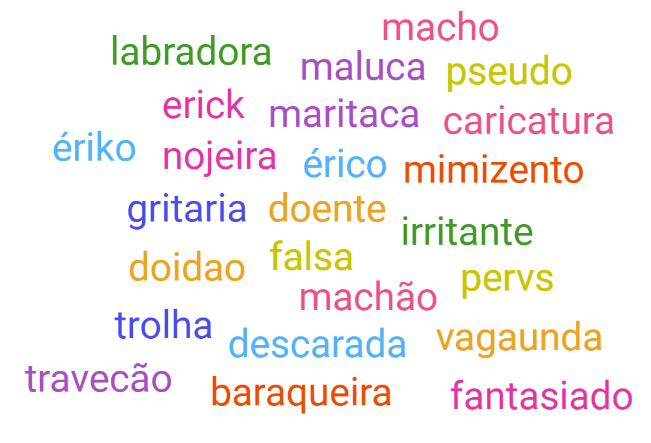
\includegraphics[width=\textwidth ]{Fig5.png}
\caption{Termos ofensivos dirigidos à deputada Erika Hilton.}
\label{fig-2}
\source{Autores, com auxílio dos programas Sketch Engine para fornecer as listas de palavras mais frequentes e Venngage para representar a lista em forma de nuvem de palavras.}
\end{minipage}
\end{figure}

A seguir, apresentamos uma amostra de dez comentários acerca do vídeo sobre o confronto entre Erika Hilton e Coronel Fernanda, ocorrido em plenário e veiculado, entre outras mídias, no YouTube. Esses comentários sugerem que críticas amargas e ataques verbais foram perpetrados contra a deputada Erika Hilton. A maioria deles, sedimentados na falsa simetria entre sexo e gênero.

\medskip
\begin{enumerate}
\item Tudo essa patifaria por falar a verdade, mulheres trans não possuem ovário, menstruação, órgãos originalmente femininos. E mulheres trans JAMAIS SERÃO mulher de verdade. E sim a sua aparência
\item Não me representa sou mulher de verdade
\item Pode falar bonito, mas vcs não são MULHERES BIOLÓGICAS, não adianta, vcs precisam lutar pelo espaço de vcs...o dia que vcs fizerem uma transvaginal e mostrar que vcs ovulam... aí sim.  Ok?
\item Apenas mais uma lembrancinha tudo na vida tem um preço, não é?
\item kkkk cala a boca Erika, vc acha q quer respeito, mais ñ respeita as mulheres
\item Ela não é vítima do patriarcado. Ela é o patriarcado. Só voltou vestida de mulher para recuperar o que conquistamos
\item Exatamente, mulher é mulher. Por mais que façam a transição, continuam sendo homem ou mulher
\item Mas mulher é uma coisa, mulher trans é outra
\item Vcs, são uma vergonha ...
\item Kkkkkkkkkkkkk me explica então, o que é ser mulher?
\end{enumerate}
\medskip

Como atestam os exemplos (1-10), para líderes de extrema direita, como a deputada Coronel Fernanda, e seus potenciais apoiadores, as conquistas das chamadas minorias sexuais representam um risco aos direitos de uma maioria fictícia e contrariam sua visão de mundo. Ao contrário da deputada Sâmia Bomfim, que foi principalmente atacada com insultos associados à aparência física e ao equilíbrio mental, os ataques à deputada Erika Hilton tomaram a forma, em sua maioria, de críticas contundentes e de demonstrações de superioridade. Como a crítica tende a ter um efeito desmoralizante, ela geralmente é vista como causa de sofrimento emocional e psicológico para o indivíduo ou o grupo alvo. Com base nesse fundamento, \textcite{culpeper2010, culpeper2011} defende que a crítica, principalmente quando amarga, é uma expressão de impolidez. Mais especificamente, em nossos dados, as críticas refletiram não apenas um tipo de avaliação negativa ao discurso de Erika Hilton no vídeo analisado, no qual ela rebate as opiniões transfóbicas da Coronel Fernanda, mas também uma tentativa de a desqualificar como uma mulher trans, uma vez que, conforme mencionado anteriormente, quase metade das críticas vieram acompanhadas de insultos à deputada.

Sintomático disso é o comentário (9), (``Vcs, são uma vergonha''). Conforme \textcite[p. 138]{elias2011}, ``O sentimento de vergonha é evidentemente uma função social modelada segundo a estrutura social''. Sendo assim, a vergonha do comentarista pela existência de um grupo (não por acaso, o sujeito do enunciado está no plural (``Vcs'')) é motivada pela percepção de que há outras estruturas sociais modelando outras formas de agir e ser, o que, para ele, é intolerável e motiva, ao mesmo tempo, o sentimento de vergonha e o ato de impolidez.

Com isso, os comentários sedimentam preconceitos e reforçam a estigmatização de pessoas LGBT+. A deputada é retratada, principalmente, como incapaz de representar as ``mulheres de verdade'', ecoando as observações da deputada Coronel Fernanda (``Não me representa, sou mulher de verdade''), como mostram os exemplos (1), (2), (3), (7) e (8). Nessa linha, nos exemplos (5) e (6), as expressões de impolidez, tais como críticas contundentes e desprezo (ou demonstrações de superioridade), também foram empregadas para descrever a conduta verbal de Erika Hilton como ``patriarcal'', em uma tentativa de forjá-la como uma ``inimiga das mulheres de verdade''.

Como também pode ser observado na reação pública ao vídeo de Erika Hilton, vários comentários refletem e contribuem para a disseminação de desinformação sobre os conceitos de ``sexo'' e ``identidade de gênero'', que são deliberadamente apresentados como equivalentes, o que se configura em uma forma de captura discursiva da terminologia \cite{lewin2021}. A prática apresenta destaque no discurso de líderes autoritários e de seus seguidores e consiste, basicamente, na subversão da linguagem e da terminologia para criar inimigos. O recurso pode ser identificado, por exemplo, quando, em nome de uma suposta ordem moral, líderes autoritários e seus seguidores transformam um transgressor em vítima, em uma estratégia também associada à ``inversão de vítima/perpetrador'', empregada para forçar uma comparação entre agentes ou circunstâncias não comparáveis e, assim, manipular a opinião pública prol de interesses específicos.

Perguntas desafiadoras também se destacaram em alguns comentários sobre a deputada Erika Hilton, por exemplo, em (4) ``Apenas mais uma lembrancinha, tudo na vida tem um preço, não é?'' e (10) ``Kkkkkkkkkkkkk me explica então, o que é ser mulher?''. Esses tipos de perguntas espelham julgamentos negativos e se alinham ao quadro teórico de \textcite{culpeper2010, culpeper2011}, no qual o autor define e exemplifica as fórmulas (ou expressões) de impolidez.

Além disso, como o anonimato tende a levar à redução da autorregulação e ao aumento de comportamentos negativos nas redes digitais, o sarcasmo e o deboche – que configuram a impolidez jocosa – desempenham um papel significativo em amplificar a severidade da crítica, ainda que de forma menos explícita, ou implicada. Em nossos dados sobre a deputada Erika Hilton, as ocorrências de sarcasmo também foram importantes por pelo menos duas outras razões interessantes. Por um lado, o sarcasmo operou como um recurso para ``debochar'' da deputada e depreciá-la por não ser uma ``mulher biológica''. Por outro lado, ele foi utilizado para disfarçar a ofensa verbal, servindo como uma estratégia antecipada para evitar a culpa em caso de incidentes legais, como também verificamos nos dados sobre a deputada Sâmia Bomfim.

\subsection{Ministra Cármen Lúcia Antunes Rocha}
Durante o julgamento que tornou o ex-presidente Bolsonaro inelegível por 8 anos, a partir de junho de 2023, coube à ministra do TSE (Tribunal Superior Eleitoral) Cármen Lúcia Antunes da Rocha dar o voto decisivo. As notícias sobre o episódio repercutiram nas redes sociais e foram intensamente comentadas. No X/Twitter, a ``\#BolsonaroInelegível'' figurou como a \textit{hashtag} mais empregada no dia do julgamento (30/06/2023), reunindo mais de 334.461 tweets. Da mesma forma, ``\#SomosTodosBolsonaro'' foi a quinta \textit{hashtag} mais popular na plataforma, ocupando essa posição por 6 horas consecutivas. Até mesmo no dia seguinte à decisão, ``\#BolsonaroInelegível'' continuou a figurar entre os tópicos mais comentados do X/Twitter, na segunda posição no país, com 440.524 \textit{tweets}. O vídeo contendo a declaração pública da ministra Cármen Lúcia sobre o julgamento também viralizou na plataforma, alcançando mais de 500 mil visualizações.

No YouTube, as duas postagens mais acessadas sobre o evento (um vídeo longo e outro curto, com recortes da fala da ministra) somaram mais de 120 mil visualizações e aproximadamente 1,3 mil comentários totais. Como esperado, a busca no Google Trends pelo nome da ministra atingiu seu pico nessa data, conforme mostra a Figura \ref{graf-4}.

\begin{figure}[h!]
\centering
\begin{minipage}{.90\textwidth}
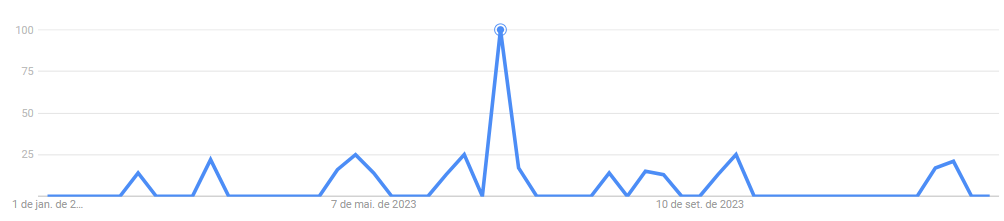
\includegraphics[width =\textwidth]{Fig6.png}
\caption{Pico de interesse público na busca pelo nome da ministra Cármen Lúcia Antunes Rocha.}
\label{graf-4}
\source{Plataforma \textit{online} Google Trends.}
\end{minipage}
\end{figure}

Seguindo o mesmo procedimento metodológico descrito nas seções anteriores, os comentários dos usuários sobre esse evento foram extraídos e analisados a fim de identificar aqueles com impolidez direcionada à ministra. Do total, 37\% dos comentários expressaram alguma forma de impolidez. Dessas postagens impolidas, 66,1\% tinham como alvo a ministra e seus supostos aliados e 33,9\% atacavam outras figuras políticas e/ou instituições representadas como adversárias. Em seguida, analisaram-se minuciosamente os comentários com impolidez dirigidos à ministra Cármen Lúcia Antunes Rocha (totalizando 553 posts retirados do YouTube e do X/Twitter) quanto ao tipo de ataque verbal. Os resultados podem ser observados nos dados da Figura \ref{graf-5}.

\begin{figure}[h!]
\centering
\begin{minipage}{.70\textwidth}
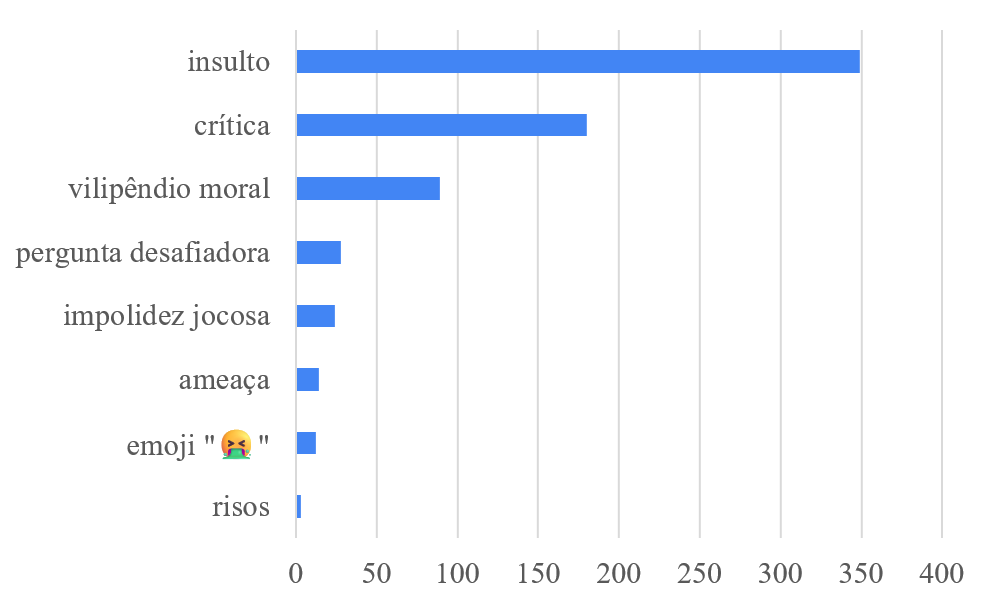
\includegraphics[width =\textwidth]{Fig7.png}
\caption{Formas de ataque mais frequentes à ministra Cármen Lúcia Antunes Rocha.}
\label{graf-5}
\source{Elaboração própria.}
\end{minipage}
\end{figure}

O insulto foi a forma mais frequente de ofensa, seguido pelas críticas, que majoritariamente estavam associadas ao fato de o presidente Lula ter sido ``inocentado'' e o ex-presidente Bolsonaro ``condenado'', segundo a visão de alguns comentaristas. Muitas vezes, na categoria crítica, os usuários atacaram a ministra Cármen Lúcia e os demais ministros, alegando perseguição e corrupção, argumentando que o evento não passava de uma ``cena'', em que tudo estaria ``armado'' e que os ministros estariam ``comprados''. Além disso, a categoria ``vilipêndio moral'' referiu-se a uma particularidade dos dados sobre Cármen Lúcia, nos quais os usuários repetidamente tentaram expor a ministra por meio de vilipêndio \textit{online}. Nesse ponto, é interessante notar que o termo ``vergonha'' foi a segunda palavra lexical mais frequente no Corpus de Impolidez Digital, especificamente o subcorpus com dados da ministra, perdendo apenas para ``Brasil''. Essa característica foi também corroborada pelo estudo de \textcite{oliveira2024}, que demonstrou ser esse o tipo de ataque mais frequente à conta do Supremo Tribunal Federal (STF), do qual a ministra também faz parte, entre 2022 e 2023. No estudo das referidas autoras, esses ataques foram perpetrados principalmente por meio da hashtag ``\#STFVergonhaNacional'', amplamente empregada em postagens no período analisado. De forma similar, nos dados sobre o banimento eleitoral do ex-presidente Jair Bolsonaro, foi observado que os usuários buscavam vilipendiar moralmente a ministra, principalmente por meio de insultos e de críticas amargas – os dois recursos que mais frequentemente acompanharam o vilipêndio moral, contabilizando 37\% e 21\% das ocorrências, respectivamente.

Em grande parte, como pode ser observado na Figura \ref{fig-3}, foram usados termos tais como ``bruxa'', ``velha'' e ``vampira'' para insultar a ministra Cármen Lúcia Antunes Rocha. Foram registrados ainda insultos dirigidos ao coletivo de ministros, insultos realizados por termos tais como ``bando de corvo'', ``urubus'' e ``corruptos''.

\begin{figure}[h!]
\centering
\begin{minipage}{.60\textwidth}
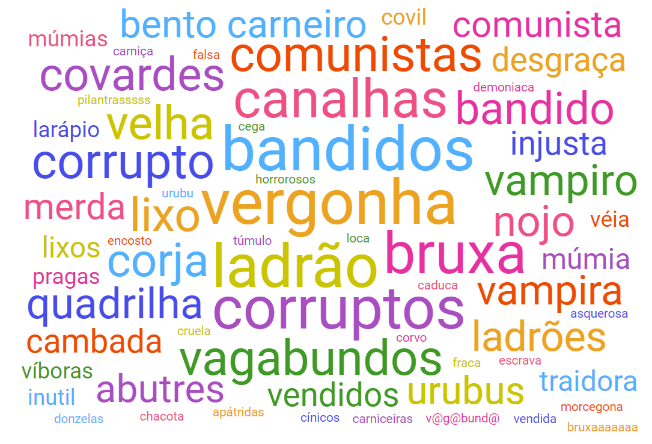
\includegraphics[width=\textwidth ]{Fig8.png}
\caption{Termos ofensivos mais frequentes dirigidos à ministra Cármen Lúcia Antunes Rocha.}
\label{fig-3}
\source{Autores, com auxílio dos programas Sketch Engine para fornecer as listas de palavras mais frequentes e Venngage para representar a lista em forma de nuvem de palavras. No gráfico, quanto mais frequente o insulto, maior o tamanho da fonte da palavra.}
\end{minipage}
\end{figure}

A esse respeito, é relevante observar duas outras categorias frequentes nos dados: o \textit{emoji} de vômito (``{\Symbola 🤮}'') e as tentativas de ameaça. Com relação ao primeiro, foram contabilizados nessa categoria os comentários sem texto, que faziam apenas o uso do \textit{emoji} de vômito repetidas vezes, seja sozinho ou associado a ``{\Symbola 🤢}''. Entretanto, houve várias ocorrências desse \textit{emoji} junto a críticas e insultos, transformando-o no terceiro item lexical mais frequente nos dados. As ameaças, por sua vez, eram apresentadas por meio de expressões tais como ``vocês vão pagar'' ou referências à ``justiça divina'', tendo como alvo tanto a ministra quanto os demais membros do TSE e do STF.

Ataques verbais fazem parte de um recurso, comum em governos de inclinação autoritária, de buscar enfraquecer a democracia e o Estado Democrático de Direito, pela manipulação da opinião pública. Nessa linha, o referido estudo de \textcite{oliveira2024} identificou uma combinação de discurso populista e de linguagem impolida e indecorosa, que circulou intensamente nas redes sociais brasileiras, particularmente no X/Twitter. Esse tipo de discurso também atua na direção da obtenção de ganhos políticos derivados da desmoralização daqueles vistos como opositores, caso dos membros do judiciário, além de contribuir para tentar criar um ambiente de tumulto, que favorece a ascensão autoritária. No caso de juízas mulheres, como ocorre com a ministra Cármen Lúcia Antunes Rocha, os limites da liberdade de expressão e da ofensa verbal, em sua relação com o princípio da dignidade humana, ficam bastante obscurecidos. Essa zona cinza pode ser observada nos exemplos de (1) a (10).
\medskip
\begin{enumerate}
    \item Carmem Lúcia, Bruxa, saída de um filme de terror
    \item Carmem Lucia vestida com sua capa preta e a cara do Bento Carneiro vampiro Brasileiro, e um adorno de presépio, uma mulher frágil e fraca, não tem personalidade própria, vai para onde o vento for. Triste ter uma Ministra da mais alta corte desse nível baixo.
    \item Nojoooo {\Symbola 🤮🤮🤮🤮}
    \item Véia loca, já morreu, só falta enterrar.
    \item Para perseguir os Processos andam rápido né TSE?
    \item Quantos vagabundos que vivem de nossos impostos e só trabalham contra o povo Carminha pega uma vassoura e voe até guantanamo vergonha das mulheres brasileiras
    \item ÉSSA FILHOTE DE CRUZ CREDO, FAZ PARTE DOS CUPINCHAS DO LADRA O QUE ELES ELEGERAM
    \item Que vergonha ministra gaguejando de tanto rolo uma senhora devia ter vergonha tão velha e tão......
    \item Essa senhora tem que aposentar ja deu
    \item Ela é frágil no seu comentário, ficou claro que ela acompanha os colegas que não toleram o Bolsonaro.
\end{enumerate}
\medskip

Nesses exemplos, em que a ministra do TSE é insultada, principalmente com relação à sua aparência e reputação, como pode ser notado pelo emprego de insultos como ``bruxa'', ``ladra'' e ``véia loca'', constantes respectivamente nos comentários (1), (8), (7) e (4), além de outros insultos, tais como em (2), ``cara do Bento Carneiro vampiro Brasileiro'' (2), e ``Carminha pega uma vassoura'', em (6), nos quais se registra a tentativa de expor a ministra por meio da inserção de  elementos da cultura popular de massa, com evidente conotação depreciativa para a maioria dos falantes de português brasileiro.

Os ataques à ministra também alvejam suas capacidades mentais e seu equilíbrio psicológico: ``uma mulher frágil e fraca, não tem personalidade própria, vai para onde o vento for. Triste ter uma Ministra da mais alta corte desse nível baixo'', em (2), e ``Ela é frágil no seu comentário, ficou claro que ela acompanha os colegas que não toleram o Bolsonaro'', em (10), que a acusam de sofrer supostas manipulações pelos demais membros (todos homens) da Corte. Há, ainda, tentativas de desqualificação da ministra por etarismo, associado ao termo ``véia'' e ``Essa senhora tem que aposentar já deu'', presentes em (4), (8) e (9).

Como os nossos dados demonstram, as tentativas de vilipêndio moral dos membros do judiciário se tornaram uma tendência comum nas redes sociais brasileiras. Resultados similares também provêm, como já comentamos, do estudo realizado por \cite{oliveira2024}. Nessa pesquisa, ficou demonstrado que o pico de uso da ``\#STFVergonhaNacional'' ocorreu entre abril e junho de 2022, na mesma época em que o inquérito sobre fake news, que atingiu alguns líderes da extrema direita e seus associados, foi deflagrado no STF. Diante dessa constatação, as autoras mostraram como as tentativas de vilipêndio moral online dos juízes ensejavam, principalmente, uma tentativa de desacreditar as decisões do STF relativamente a esse inquérito e, possivelmente, também a outros, de forma antecipada.

Os achados sobre a ministra Cármen Lúcia Antunes Rocha e as deputadas Sâmia Bomfim e Erika Hilton são consistentes com estudos anteriores, realizados em outros países \cite{wodak2021, wodak2021culpeper}, que reafirmam o fenômeno da agressão verbal contra mulheres, mesmo aquelas em posição de influência, como um traço importante da esfera digital. Esses resultados também sugerem que a ofensa verbal de gênero, no domínio cibernético, é alimentada, centralmente, pela fabricação, ou pela manutenção, do ciclo de ataques associado a um alvo comum, retratado como inferior. Ao obstruir o debate genuíno, é importante, mais uma vez, destacar que esse ciclo de agressão afeta o tecido social como um todo, e não apenas as mulheres, ou as pessoas LGBT+. Toda a sociedade é colocada em risco, já que a pluralidade é desafiada, provocando insegurança e tumulto.

\section{Considerações finais}\label{sec-conclusao}
Os estudos multicaso discutidos neste artigo trouxeram à luz elementos importantes para a abordagem teórico-metodológica que se pretendeu desenvolver e podem, por isso, inspirar outros estudos. A esse respeito, destacamos que os estudos da impolidez advogam que os indivíduos tendem a avaliar como ofensivos aqueles comportamentos verbais conflitantes com a conduta esperada para determinadas situações. Dito de outro modo, a percepção da impolidez é, primeiramente, dependente da situação comunicativa, ou seja, ela está circunscrita ao contexto imediato da interação \cite{culpeper2010, culpeper2011}. Para identificar esse contexto, em geral, os falantes implicitamente se perguntam: ``quem fala? o que fala? para quem fala? onde fala? por que fala? como fala?''.

No caso das mídias sociais, no entanto, a identificação desses componentes é menos nítida, em razão, por exemplo, do alegado anonimato, da possibilidade de as mensagens estarem sendo deflagradas em grande escala por um robô (\textit{bot}), além do alcance imprevisível dessas mesmas mensagens, que circulam para uma audiência abstrata, composta quase em sua totalidade por desconhecidos. A esses elementos, somam-se ainda a informalidade e a sensação de proximidade, mesmo mediante estranhos, além da velocidade da reprodução, bem como dos componentes multimodais (verbais, não verbais e híbridos), que acrescentam complexidade ao texto digital.  

No episódio envolvendo as duas deputadas, em relação ao contexto imediato, é de se supor que a função parlamentar seja condizente com o chamado ``decoro'', pelo qual é esperado um comportamento verbal respeitoso e diplomático de líderes políticos, principalmente quando eles se dirigem em público (seja \textit{online} ou em presença física), a uma colega, em pleno exercício de sua função. Nesse sentido, o emprego de algumas expressões, ou fórmulas, indica que a impolidez foi exercida, caracterizando a ofensa. A percepção da ofensa, nos casos estudados, foi, portanto, fortemente baseada em uma quebra da ordem moral vigente. Ela foi também marcada pelo emprego de insultos, críticas amargas e de sarcasmo, este último aplicando um tom deliberadamente jocoso aos comentários, que facilita a sua reprodução na esfera digital e antecipa uma possível evasão da culpa, em caso de incidentes legais.

Em suma, críticas ao judiciário e a agentes públicos em geral são esperadas e legítimas em uma sociedade democrática. Elas são, no entanto, muito distintas de ofensas, difamações e falsas acusações, em geral produzidas em busca de obtenção de vantagens circunstanciais. É nesse sentido que a proteção de mulheres e de pessoas LGBT+ inclui uma dimensão discursiva crucial, associada à preservação do Estado Democrático de Direito. A tarefa deve ser de todas e de todos, já que a todas e a todos afeta, ainda que de formas e em intensidades diversas.

\section*{Agradecimentos}
Agradecemos aos membros do Projeto ``Discurso Digitalmente Mediado da Extrema Direita no Brasil e seus Efeitos nos Direitos Humanos de Mulheres, Meninas e da Comunidade LGBT+'' (CNPq – Processo número 404672/2023-0) pelas importantes contribuições nas várias fases de produção deste estudo. Também gostaríamos de agradecer aos avaliadores anônimos pelos comentários valiosos, que nos ajudaram a melhorar o texto. Registramos ainda nossos agradecimentos ao CNPq pela concessão da Bolsa Produtividade em Pesquisa aos pesquisadores Ana Larissa Adorno Marciotto Oliveira (processo 307538/2023-0) e Gustavo Ximenes Cunha (processo 304805/2022-0), bem como pela Bolsa de Pós-Doutorado (processo 151002/2024-0) concedida a Monique Vieira Miranda.



\printbibliography\label{sec-bib}
% if the text is not in Portuguese, it might be necessary to use the code below instead to print the correct ABNT abbreviations [s.n.], [s.l.]
%\begin{portuguese}
%\printbibliography[title={Bibliography}]
%\end{portuguese}


%full list: conceptualization,datacuration,formalanalysis,funding,investigation,methodology,projadm,resources,software,supervision,validation,visualization,writing,review
\begin{contributors}[sec-contributors]
\authorcontribution{Ana Larissa Adorno Marciotto Oliveira}[conceptualization,supervision,investigation,methodology,writing,review]
\authorcontribution{Monique Vieira Miranda}[formalanalysis,investigation,methodology,writing]
\authorcontribution{Tímea Drinóczi}[formalanalysis,investigation,writing]
\authorcontribution{Gustavo Ximenes Cunha}[writing,review]
\end{contributors}


\
\end{document}

